\section{Convolutional Neural Network} \label{sc:cnn}
Bisher wurden in erster Linie die Grundlagen für die heutigen neuronalen Netze erläutert. Im kommenden Abschnitt werde ich grob darauf eingehen wie man diese Techniken nutzen kann um mithilfe eines \emph{Convolutional Neural Networks} Bilder zu erkennen. 


\subsection{Geschichte}

\paragraph{Zellarten} 
Im Jahr 1959 entdeckten die beiden Neurophysiologe Torsten Wiesel und David H. Hubel die sogenannten \emph{simple} und \emph{complex cells}. Sie beschrieben einen groben Zusammenhang dafür wie diese beiden Zellarten bei der Mustererkennung im visuellen Kortex verwendet werden. 

\begin{itemize}
\item Die \emph{simple cells} können einfache Kanten und Balken mit einer bestimmten Orientierung erkennen. Ein solche Zelle könnte zum Beispiel in der Lage sein einen Balken am unteren Bildrand als solchen zu erkennen. 

\item Eine \emph{complex cell} ist ebenfalls dazu in der Lage diese Formen zu erkennen allerdings mit dem Zusatz diese Konstellation von Formen auch an verschiedenen Positionen des Bildes zu erkennen. Bezogen auf das Beispiel vom letzten Punkt könnte diese Zellart auch in der Lage sein solche Balken in der Mitte oder am oberen Rand des Bildes zu erkennen. Diese Eigenschaft der Positionsunabhängigkeit eines Musters wird \emph{spatial invariance} genannt (zu deutsch \glqq räumliche Invarianz\grqq ).
\end{itemize}

Einige Jahre später (1962), beschrieben die beiden Wissenschaftler wie genau solche komplexen Zellen diese Eigenschaft erreichen. Diese Zellen summieren die Ausgaben von mehreren \emph{simple cells} auf. Alle beteiligten Zellen sind auf die gleichen Formen spezialisiert, analysieren jedoch jeweils einen unterschiedlichen Teil des Bildes (englisch \emph{receptive fields}, siehe Abbildung \ref{fig:simpleVsComplex}). So kann zum Beispiel eine komplexe Zelle horizonale Balken an mehreren Positionen im Bild erkennen indem sie auf die unterschiedlichen Ausgabewerte von mehreren simplen Zellen zurückgreift und diese aufaddiert. Diese Herangehensweise des Herunterbrechens einer komplexen Aufgabe in mehrere einfachere Aufgaben ist ein wesentliches Merkmal aller neuronalen Netze sowie der menschlichen Wahrnehmung im visuellen Kortex. 

\begin{figure}[!htb]
	\centering
	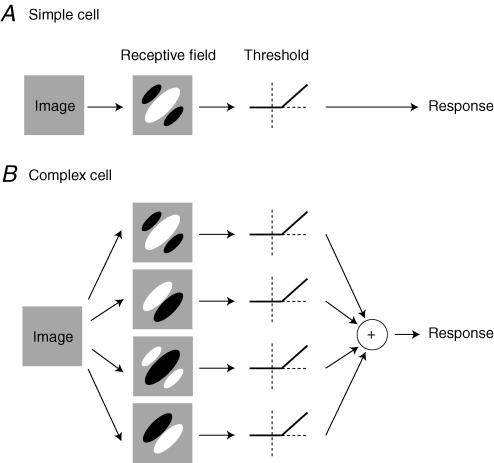
\includegraphics[width=.6\linewidth]{img/simpleVsComplex}
	\mycaption{Vergleich  - Simple und Complex Cell}{cnnHistory}
	\label{fig:simpleVsComplex}
\end{figure}

In den 1980er Jahren entwickelte Dr. Kunihiko Fukushima das Modell von Hubel und Wiesel weiter indem er ein mathematisches Modell mit den beiden Typen \emph{S-Cells} und \emph{C-Cells} einführte. Die S-Cells befinden sich jeweils in der ersten Schicht des Modells und sind mit den C-Cells verbunden. 

\paragraph{Erkennung von Handschrift}
Einer der Pioniere auf dem Gebiet ist der französische Informatiker Yann LeCun. In den 90er Jahren publizierte er diverse Ausarbeitung. In seiner bekanntesten beschreibt er wie ein einfaches CNN Modell in der Lage ist handschriftliche Ziffern zu erkennen. Sein Modell verwendet wie schon angedeutet die Eigenschaft mit einfach Formen komplexere zu bilden und somit die Ziffern zu erkennen. Um sein Modell zu trainieren verwendete er die \emph{MNIST database of handwritten digits}. Diese Datenbank enthält Bilder von handgeschriebenen Ziffern welche jeweils mit einem entsprechenden Label versehen wurden. Diese Daten werden vom Netz verwendet um die Kostenfunktion aufzustellen\footnote{Es sei ebenfalls noch kurz erwähnt, dass es zu sehr vielen Themengebieten derartige Datenbanken gibt. Eine umfangreiche Liste von frei verfügbaren Quellen ist hier \cite{openDataSets} zu finden.}. Die Datenbank enthält circa 60.000 Datensätze welche ausschließlich zum trainieren des Netzes verwendet werden und 10.000 Datensätze um den letztendlichen Fehler zu berechnen. Wie genau dies geschieht wird im späteren Verlauf des Kapitels geklärt (siehe \emph{Backpropagation} Kapitel \ref{sec:backprop}).

\subsection{Funktionsweise}
Gegeben sei ein beliebiges Bild, ein CNN soll nun in der Lage sein dazu anzugeben mit welcher Wahrscheinlichkeit das Bild zu einer definierten Klasse gehört. Dies können durchaus auch mehr als eine Klasse pro Bild sein. Das zu kategorisierende Bild wird in Form einer Matrix verarbeitet. In Abbildung \ref{fig:puppies} kann man grob erkennen wie so etwas aussehen könnte.

der folgenden Darstellung kann man grob sehen wie sowas in etwa aussehen könnte (). 

\begin{figure}[!htb]
	\centering
	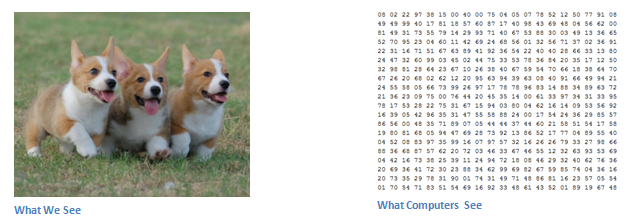
\includegraphics[width=.9\linewidth]{img/humanVsPc}
	\mycaption{Vergleich  - Darstellung Mensch und Maschine}{cnnExplained}
	\label{fig:puppies}
\end{figure}

Die rechte Darstellung ist hierbei auch noch unvollständig, denn es handelt sich bei dem Bild um ein Farbbild. In der Praxis werden für jedes Pixel drei unterschiedliche Farbwerte zwischen 0 und 255 gespeichert (wenn man sich im RGB-Farbraum befindet). Um die Ausgabeklasse eines Eingabearrays zu bestimmen wird wie schon bei den vorherigen Modellen darauf gesetzt von \emph{low-leve}l Eigenschaften, wie bestimmte Formen an bestimmten Positionen, auf \emph{high-level} Eigenschaften geschlossen. Um dies zu erreichen wird bei dieser Art von Netz mit mehreren sogenannten Layern gearbeitet. Das Modell besteht im wesentlichen aus zwei Arten von Schichten: den Filtern (\emph{convolutional layer}) und Aggregations-Schichten (\emph{Pooling Layer}). Diese wiederholen sich abwechselnd. In Abbildung \ref{fig:cnnOverview} ist zu erkennen wie die beschriebenen Zwischenschritte der Verarbeitung grob aussehen können. 

\begin{figure}[!htb]
	\centering
	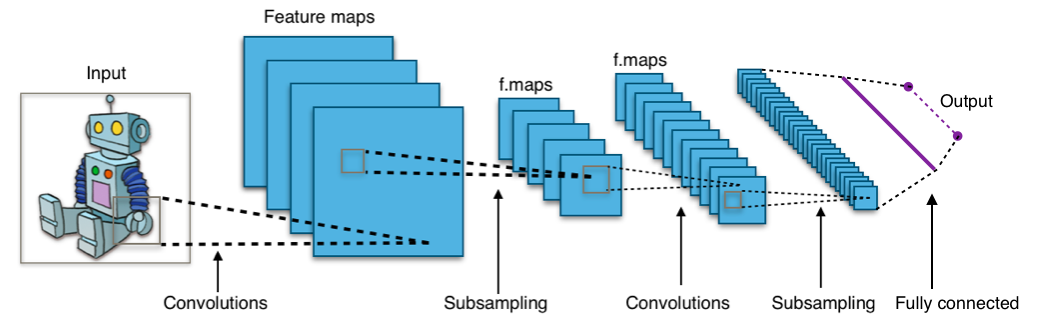
\includegraphics[width=.9\linewidth]{img/cnn_overview}
	\mycaption{Überblick - CNN Verarbeitungsschritte}{cnnFunktionsweise2}
	\label{fig:cnnOverview}
\end{figure}

\paragraph{Convolutional Layer}
Der gegebene Matrix-Input wird mittels sogenannter \emph{Filter} (auch \emph{Neuron} oder \emph{Kernel} genannt) analysiert. Ein Filter besitzt eine feste Pixelgröße (\emph{Kernel-Size}) wie zum Beispiel 5 x 5. Diese spannt ein kleines \glqq Fenster\grqq  über der Matrix auf. Dieses Fenster wandert beziehungsweise scannt anschließend mit einer definierten Schrittweite zeilenweise die Eingabematrix. Mittels eines Parameters \emph{Padding} wird festgelegt, wie sich der Filter verhalten soll wenn er den Rand der Matrix erreicht. Die betrachteten Pixel im Betrachtungsfenster aggregieren zu einem Neuron in der nächsten Schicht. Die Abbildung \ref{fig:cnn_convLayer} zeigt in relativ verständlicher Weise wie der sogenannte erste \emph{hidden Layer} dadurch aufgebaut wird. Wichtig: \emph{Die Größe dieser Ergebnismatrix ist abhängig von der Größe (Kernel-Size) des Filters, dem Padding und vor allem von der Schrittweite} \cite{cnnFunktionsweise2}. 

\begin{figure}[!htb]
	\centering
	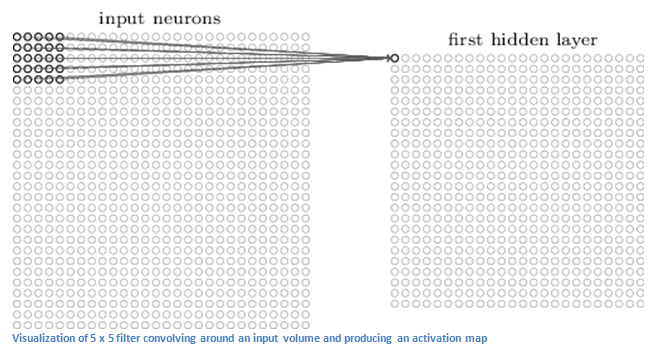
\includegraphics[width=.6\linewidth]{img/cnn_convLayer}
	\mycaption{CNN - Convolution Layer}{cnnFunktionsweise2}
	\label{fig:cnn_convLayer}
\end{figure}

Eine Schrittweite von 2 bei einem Betrachtungsfenster von 2 x 2 Pixeln fúhrt beispielsweise pro Filter zu einer Halbierung der Größe der Ergebnis-Matrix im Vergleich zur Input-Matrix. Da in diesem Beispiel immer 4 Pixel gleichzeitig an einem Filter \glqq hängen\grqq  wird die Eingabe in gewisser Weise \emph{gefaltet} (englisch \emph{convolution}). 

In der Praxis wird oft ein convolutional Layer mit 32 oder 16 Bit Filtern verwendet. Jeder dieser Filter generiert eine eigene Ausgabematrix. Als nächste Schicht folgt erneut ein convolutional Layer welcher die Ausgabematrizen als neuen Input verwendet. Die dadurch generierte Ausgabe wird auch \emph{activation map} oder \emph{feature map} genannt und wird wiederum in einen \emph{Pooling Layer} gesteckt. 

\subparagraph{Beispiel - Handschriftliche Ziffern}
Im folgenden Beispiel betrachten wir die Erkennung einer Ziffer 7 (siehe Abbildung \ref{fig:cnn_filter}).Diese Ziffer besteht aus mehreren Bestandteilen. Es gibt zum Beispiel einen vertikalen Strich von Links unten nach rechts oben, manche schreiben auch noch einen Querstrich in die Mitte der Ziffer. In diesem Einschub wollen wir uns aber dem Querstrich im oberen Teil der 7 widmen. 

\begin{figure}[!htb]
	\centering
	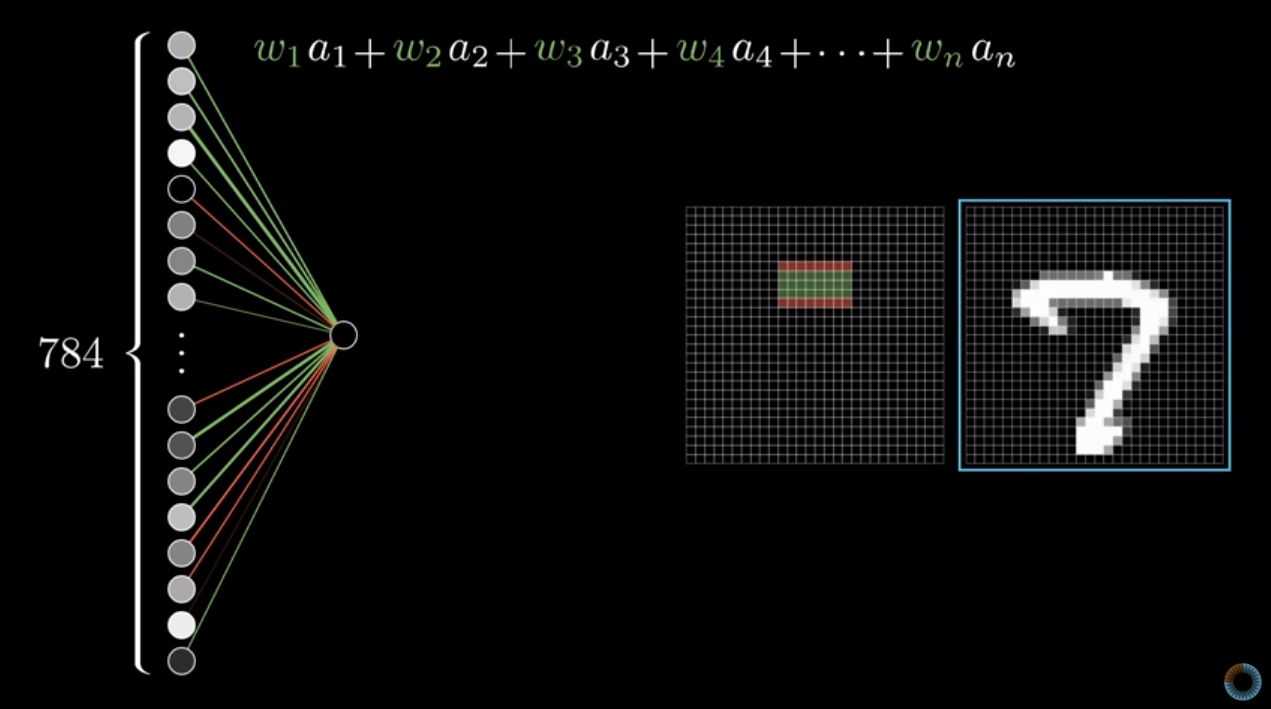
\includegraphics[width=.7\linewidth]{img/filter}
	\mycaption{CNN - Filter}{3b1b}
	\label{fig:cnn_filter}
\end{figure}

Um diese Ziffer 7 als eine solche zu erkennen muss das Netz in der Lage sein unter anderem diesen Querstrich zu erkennen. Um diese Eigenschaft zu erkennen bildet man hierfür ein Betrachtungsfenster. Jeder Pixel innerhalb dieses Betrachtungsfensters bekommt ein Gewicht zugewiesen. Die Darstellung ist so zu verstehen, dass die roten Kästen ein negatives Gewicht und die grünen ein positives Gewicht darstellen. Die schwarzen Kästen sollen dagegen ein Gewicht mit dem Wert $0$ enthalten. Wenn man nun die erhaltenen Pixelwerte (in der Abbildung rechts) mit den entsprechenden Gewichten multipliziert und aufaddiert bekommt man einen recht hohen Wert, wenn in dem gegebenen Bild ein Querstrich in diesem Teil des Bildes vorhanden sein sollte, und einen sehr kleinen wenn dies nicht der Fall ist. Durch diesen Sachverhalt ist es möglich eine primitive Eigenschaften des Bildes zu erkennen.  

Pro zu erkennenden Merkmal gibt es in einem CNN einen Filter. Jedes Betrachtungsfenster dieses Filters würde dann die erwarteten Farbwerte für die jeweilige Ziffer widerspiegeln. Die Erkenntnisse dieser \emph{low-Level} Filter können dann wiederum mit weiterführenden Filtern verarbeitet werden. Und so können nach und nach auch die komplexesten Formen erkannt werden. 

Letztendlich erinnert dieses Prinzip doch sehr stark an die Entdeckung von Hubel und Wiesel. Die einzelnen Neuronen die innerhalb dieses Netzes verwendet werden halten sich jedoch stark an die Funktionsweise des Adeline-Modells. Hierbei werden jedoch mehrere Schichten hintereinander gehängt um die Komplexität des ganzen zu steigern. 

\paragraph{Pooling Layer}
Ein \emph{Pooling Layer} ist dafür zuständig die Ergebnisse von Convolutional Layern zu aggregieren. Dies wird anhand eines Pooling-Prozesses ausgewertet. Der wesentliche Zweck dieser Schicht ist es \emph{nur die relevantesten Signale an die nächsten Schichten weiter zu geben, eine abstraktere Repräsentation des Inhalts zu erreichen und die Anzahl der Parameter eines Netzes zu reduzieren} \cite{cnnFunktionsweise2}. Generell gilt, während die Größe des Inputs durch die Faltungen und das Pooling immer weiter reduziert wird, erhöht sich die Anzahl der Filter zur Erkennung von übergeordneten Signalen zunehmend.

Ein weit verbreiteter Pooling-Mechanismus stellt der sogenannte \emph{MaxPooling Layer} dar. Hierbei wird einfach der höchste Wert einer Kernel-Matrix verwendet und alle anderen werden verworfen. Es gibt allerdings auch andere Algorithmen auf die ich hier jedoch nicht näher eingehen werden: 

\begin{multicols}{2}
\begin{itemize}
\item fractuional max pooling
\item Lp pooling
\item mean pooling
\item stoachastic pooling
\item spatial pooling
\item generalized pooling
\end{itemize}
\end{multicols}


\paragraph{Fully Connected Layer}
Diese Schicht wird auch oft als \emph{Dense Layer} bezeichnet. Ausgangspunkt für die Verwendung dieses Layers ist, dass sämtliche high-level Merkmale bereits durch die vorangegangenen Schichten erkannt wurden. In dieser Schicht werden sämtliche Neuronen mit allen Ein- und Ausgabewerten verbunden. Generell fasst diese Schicht alle high-level Merkmale zu den jeweiligen Ausgabeklassen zusammen. Wenn wir beim Beispiel der Ziffernerkennung bleiben, spiegelt die Vorgängerschicht die einzelnen Schnörkel und Striche der einzelnen Ziffern wieder. Der Dense Layer fasst diese dann zu den wirklichen Ziffern zusammen. So entsteht als Ausgabe hierbei ein N-dimensionaler Vektor welcher in den einzelnen Komponenten die jeweilige Wahrscheinlichkeit hält, dass es sich um die jeweilige Klasse handelt oder nicht. Bei den Ziffern wäre dies ein 10 dimensionaler Vektor. Wenn man nun die Ziffer 0 erkennen wollen würde kann es gut sein, dass sich das Netz \glqq nicht ganz sicher\grqq  ist, da es die Ziffer 9 im oberen Bereich zum Beispiel ebenfalls eine Rundung besitzt. Die Ausgabe könnte dann so aussehen, dass alle Komponenten bis auf die am Index 0 und 9 mit einer Wahrscheinlichkeit von 0 belegt wurden. 

\paragraph{Training} 
Um sämtliche Gewichte und Schwellwerte des Netzes richtig anpassen zu können wird auf einen Trainingsalgorithmus zurückgegriffen. Das in diesem Fall genutzte Verfahren der \emph{Backpropagation} ist von fundamentaler Bedeutung für alle aktuellen Architekturen, daher bekommt er eine eigenen Section (siehe Kapitel \ref{sec:backprop}). 
